%\setchapterimage{bandeau}
\chapter*{Colle \arabic{cptColle} \\ 
Réglage d'un correcteur P et d'un correcteur à avance de phase -- 
\ifprof Corrigé \else Sujet \fi}
\addcontentsline{toc}{section}{Colle \arabic{cptColle} :
Réglage d'un correcteur P et d'un correcteur à avance de phase -- 
\ifprof Corrigé \else Sujet \fi}

\iflivret \stepcounter{cptColle} \else
\ifprof  \stepcounter{cptColle} \else \fi
\fi

\setcounter{question}{0}
\marginnote{Equipe PT -- La Martinière Monplaisir.}
\marginnote[1cm]{
\UPSTIcompetence[2]{C1-02}
\UPSTIcompetence[2]{C2-04}}


%\begin{marginfigure} [4cm]
%\includegraphics[width=\linewidth]{fig_01a}
%\end{marginfigure}


On considère un système de fonction de transfert en boucle ouverte $G(p)$ que l'on souhaite réguler à l’aide d'une boucle à retour unitaire : $G(p)=\dfrac{K}{\left(10p+1 \right)^2\left(p+1 \right)}$

On souhaite que la boucle de régulation fonctionne selon le cahier des charges suivant :
\begin{itemize}
\item marge de phase : $\Delta \varphi \geq 45\degres$;
\item dépassement $D\% < 10\%$ ; 
\item écart statique $\varepsilon_S < 0,08$ ; 
\item temps de montée $t_m < \SI{8}{s}$.
\end{itemize}

\question{Quelle est la condition sur $K$ pour obtenir $\varepsilon_S<0,08$ ?}

On note $t_m$ le temps de montée du système en BF et $t_m\simeq \dfrac{3}{\omega_{\text{co}}}$ et $\omega_{\text{co}}$ est la pulsation de coupure à \SI{0}{dB} du système en BO.  

\question{Quelle est la condition sur $K$ pour obtenir $t_m<\SI{8}{s}$ ?}


\question{Quel choix faire pour la valeur de $K$ ?}

\question{Calculer la valeur de la marge de phase obtenue dans ces conditions. }


Expérimentalement, on constate que 
$z_{\text{BF}}\simeq \dfrac{\Delta \varphi ^{o}}{100}$ 
et on rappelle que $D\% = e^{\dfrac{-\pi z_{BF}}{\sqrt{1-z_{BF}^2}}}$.

\question{Que vaut alors le dépassement D\%?}


\question{À partir de la relation précédente, déterminer la marge de phase qui correspond à un dépassement de 10\%.}

Avec la valeur de $K=16,1$, on introduit, en amont de $G(p)$, dans la chaîne directe, un correcteur $C(p)=K_a \dfrac{1+aTp}{1+Tp}$ à avance de phase destiné à corriger le dépassement et la marge de phase, sans altérer ni la rapidité, ni la précision qui correspondent au cahier des charges.

\question{Déterminer alors la fonction de transfert de ce correcteur à avance de phase permettant d’obtenir une marge de phase de 60\degres.}



\ifprof

\begin{center}

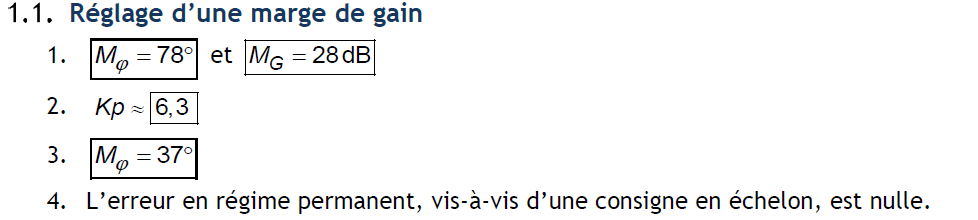
\includegraphics[width=\linewidth]{cor_01}

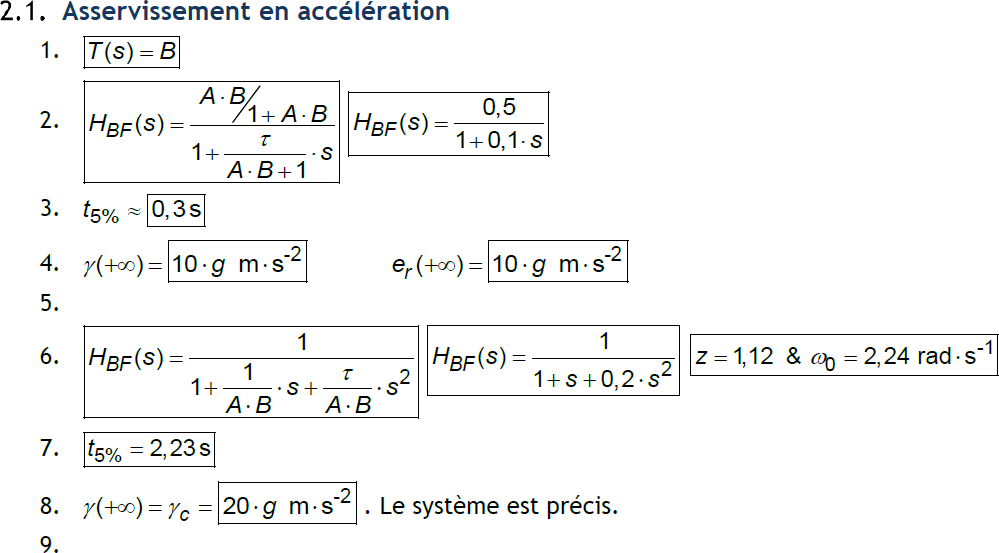
\includegraphics[width=\linewidth]{cor_02}
\end{center}
\else
\fi
